\subsection{Experiment/Results}

{
\paper{Xochicale 2019 in {\bf PhD thesis} }
\begin{frame}{Human-Humanoid Imitation Activities}
20 participants with mean and standard deviation (SD) age of 
mean=19.8 (SD=1.39) years, being four females and sixteen males.
    \begin{figure}
        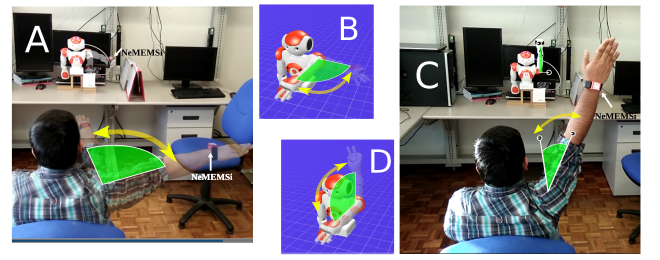
\includegraphics[width=0.9\linewidth]{./figs/experiment/versions/drawing-v00}{}
	\caption[PA]{(A/C) Front-to-Front Human-Humanoid Imitation 
		Activities of Horizontal/Vertical Movements,
		(B/D) NAO, humanoid robot, performing 
		Horizontal/Vertical arm movements.
		}
   \end{figure}
\end{frame}
}




%%%%%%%%%%%%%%%%%%%%%%%%%%%%%%%%%%%%%%%%%%%%%%%%%%%%%%%%%%
{
\paper{Xochicale 2019 in {\bf PhD Thesis}}
\begin{frame}{From Raw to Smoothed Time Series}
   \begin{figure}
        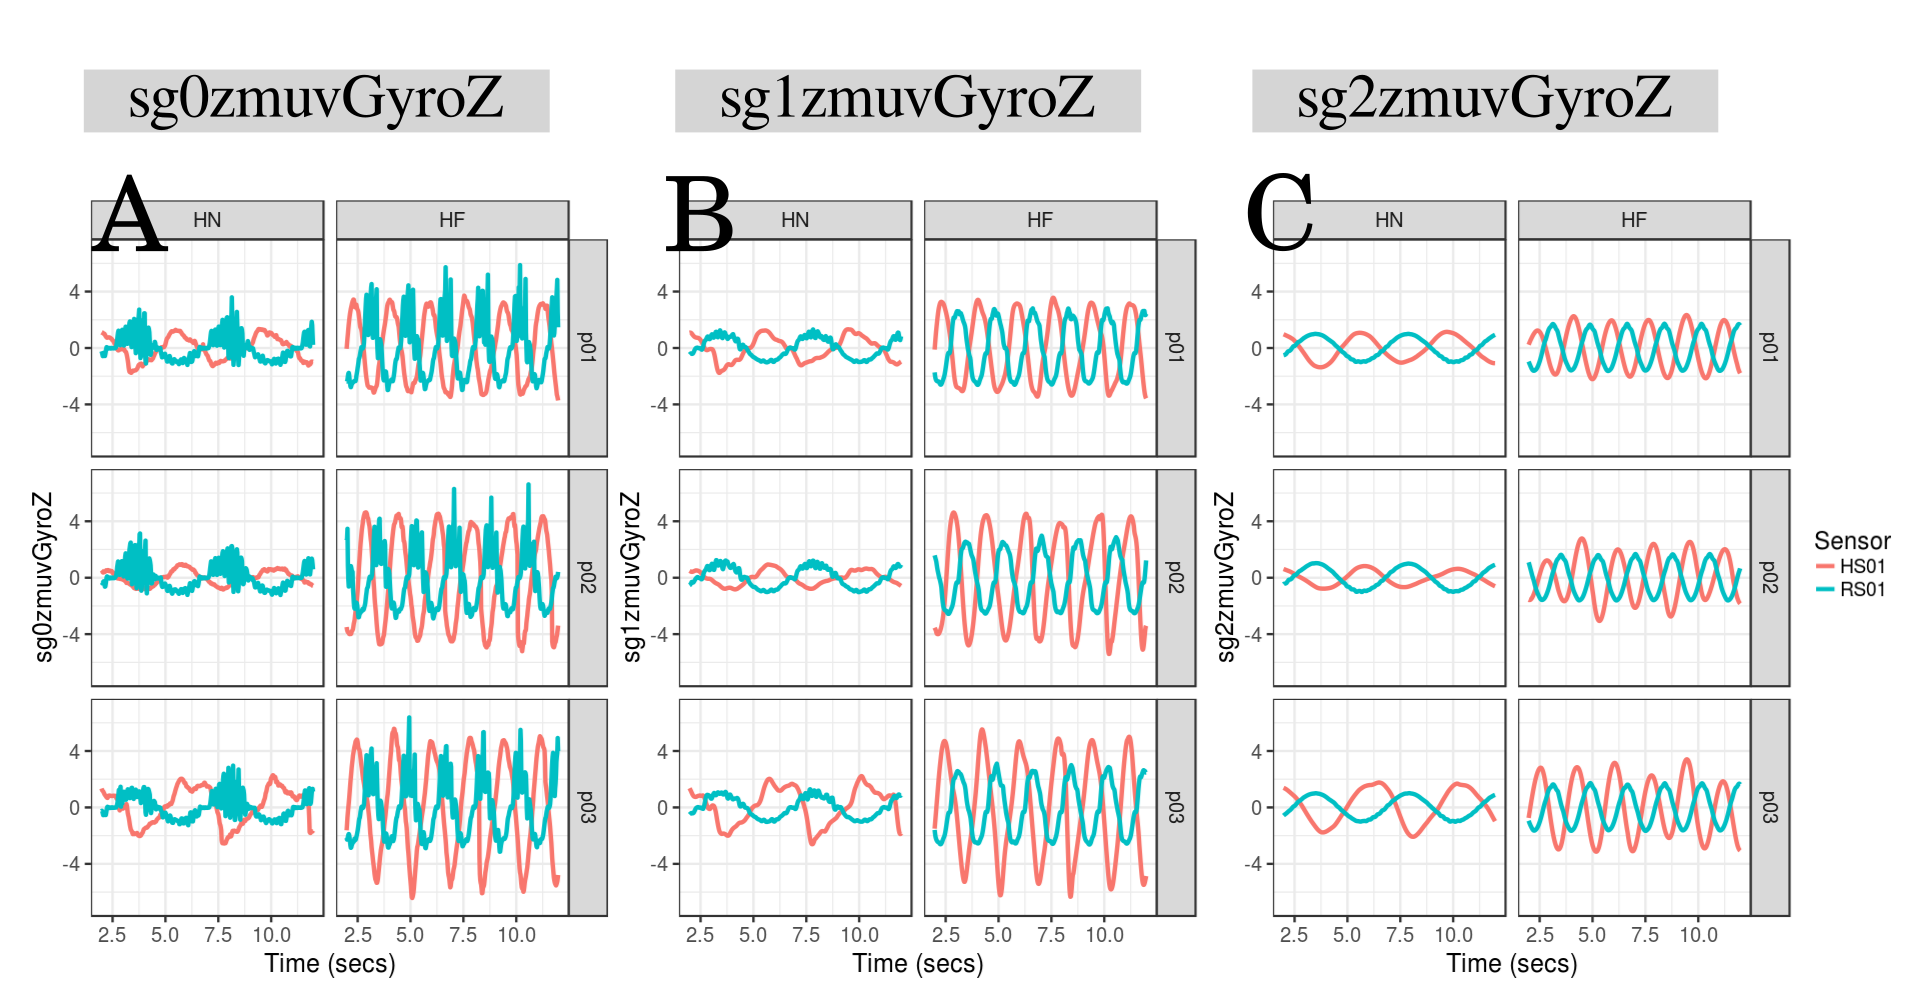
\includegraphics[width=0.9\linewidth]{./figs/results/ch6-ts-h/versions/drawing-v00}{}
	\caption{Time-series of horizontal movements for 
	(A) normalised, (B) \texttt{sgolay(p=5,n=25)}, and 
	(C) \texttt{sgolay(p=5,n=159).} } 
   \end{figure}
\end{frame}
}


%%%%%%%%%%%%%%%%%%%%%%%%%%%%%%%%%%%%%%%%%%%%%%%%%%%%%%%%%%
{
\paper{Xochicale 2019 in {\bf PhD Thesis}}
\begin{frame}{From Raw to Smoothed Time Series}
   \begin{figure}
        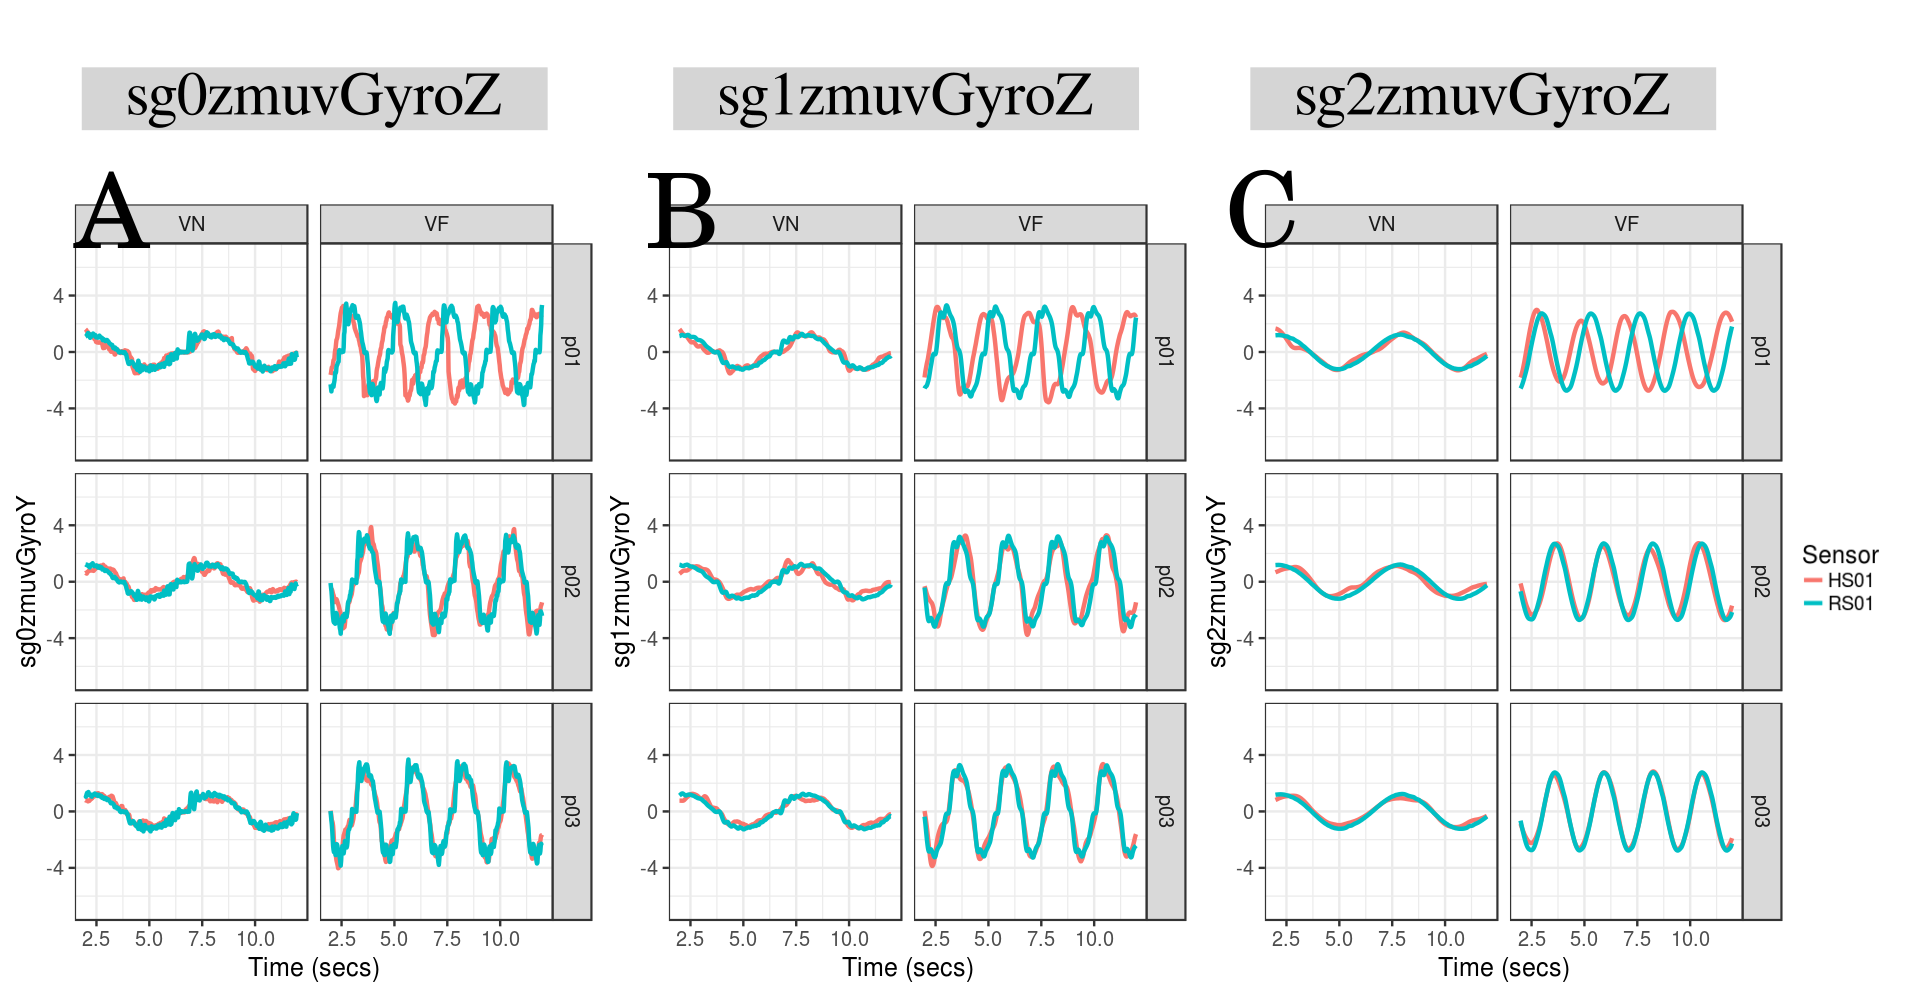
\includegraphics[width=0.9\linewidth]{./figs/results/ch6-ts-v/versions/drawing-v00}{}
	\caption{Time-series of vertical movements for 
	(A) normalised, (B) \texttt{sgolay(p=5,n=25)}, and 
	(C) \texttt{sgolay(p=5,n=159).} } 
   \end{figure}
\end{frame}
}



%%%%%%%%%%%%%%%%%%%%%%%%%%%%%%%%%%%%%%%%%%%%%%%%%%%%%%%%%
{
\paper{Xochicale 2019 in {\bf PhD Thesis}}
\begin{frame}{Minimum Embedding Parameters}
    \begin{figure}
        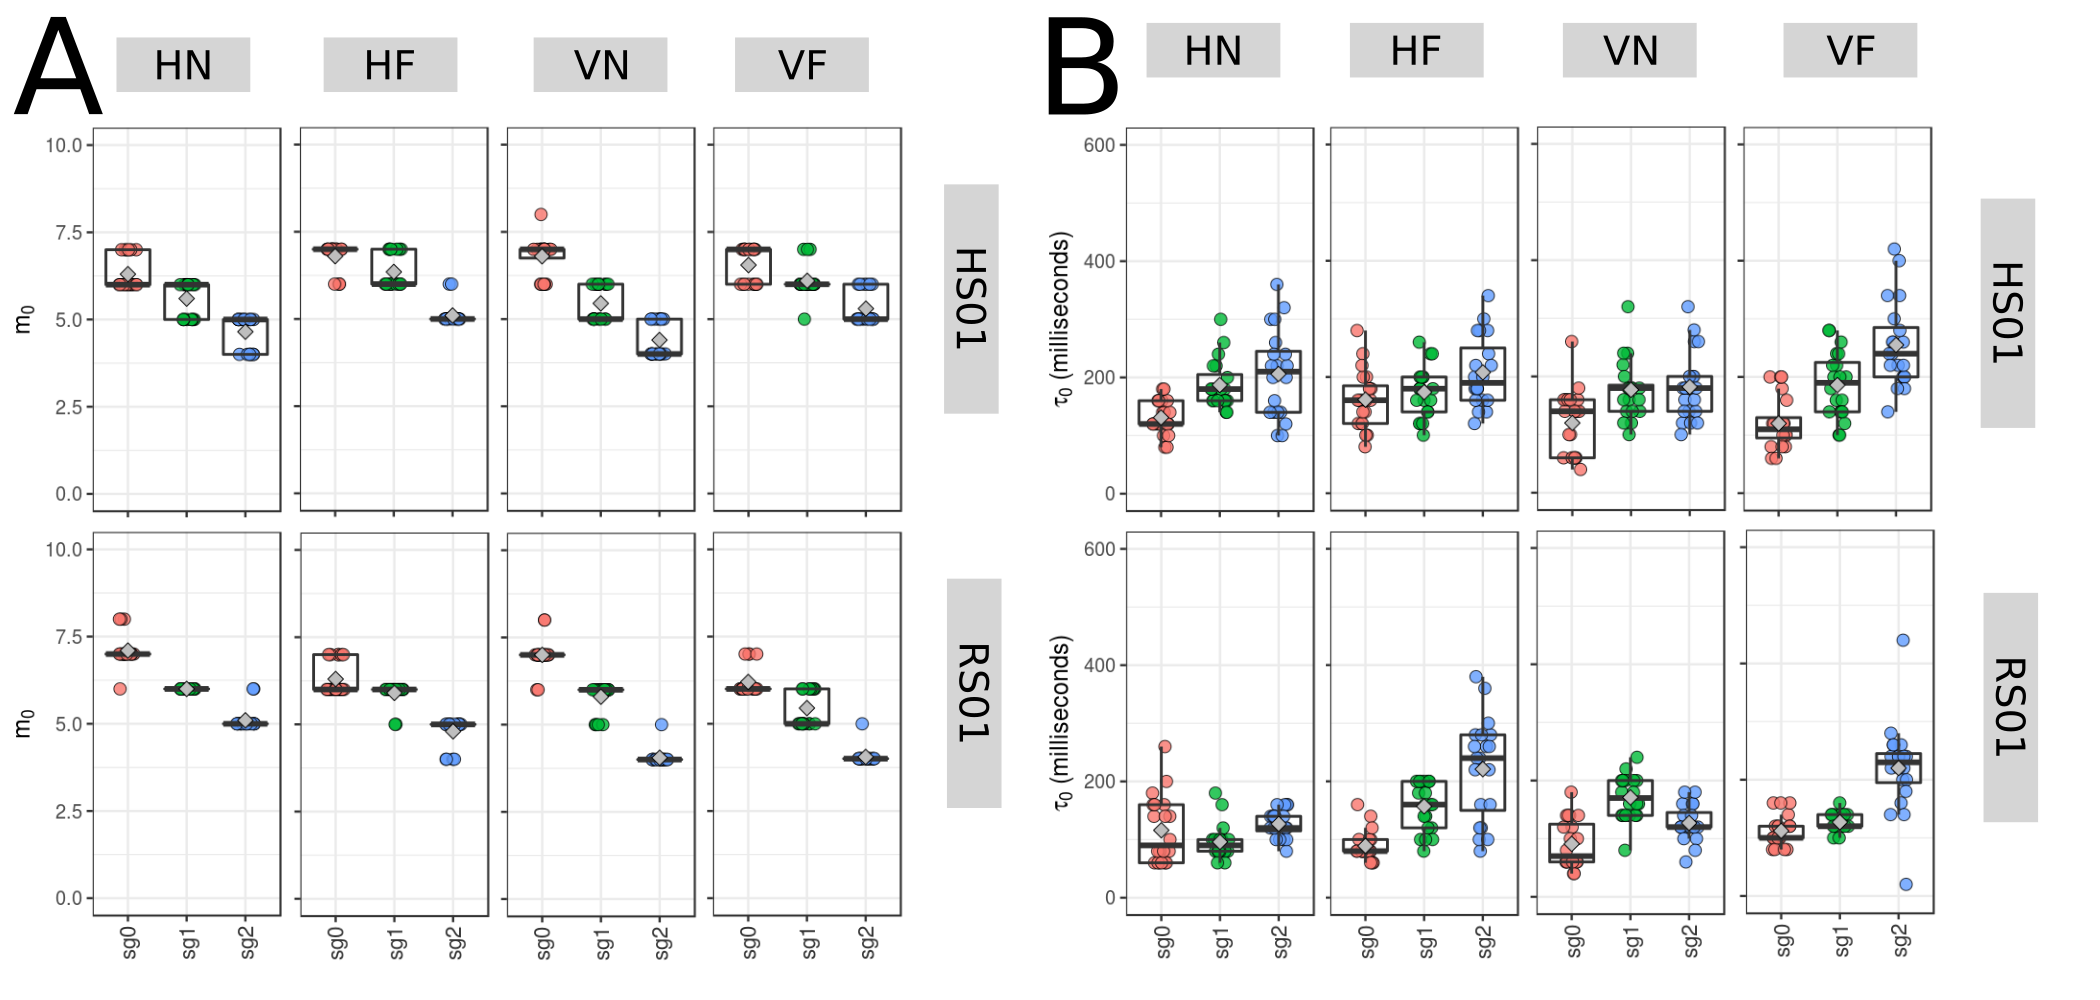
\includegraphics[width=0.9\linewidth]{./figs/results/ch6-empa/versions/drawing-v00}{}
	\caption{(A) Minimum Embedding Dimension 
		 (B) First Minimum AMI
		}  
   \end{figure}
	
\end{frame}
}


%%%%%%%%%%%%%%%%%%%%%%%%%%%%%%%%%%%%%%%%%%%%%%%%%%%%%%%%
{
%\paper{Xochicale 2019 in {\bf PhD Thesis}}
\begin{frame}{Reconstructed State Spaces}
    \begin{figure}
        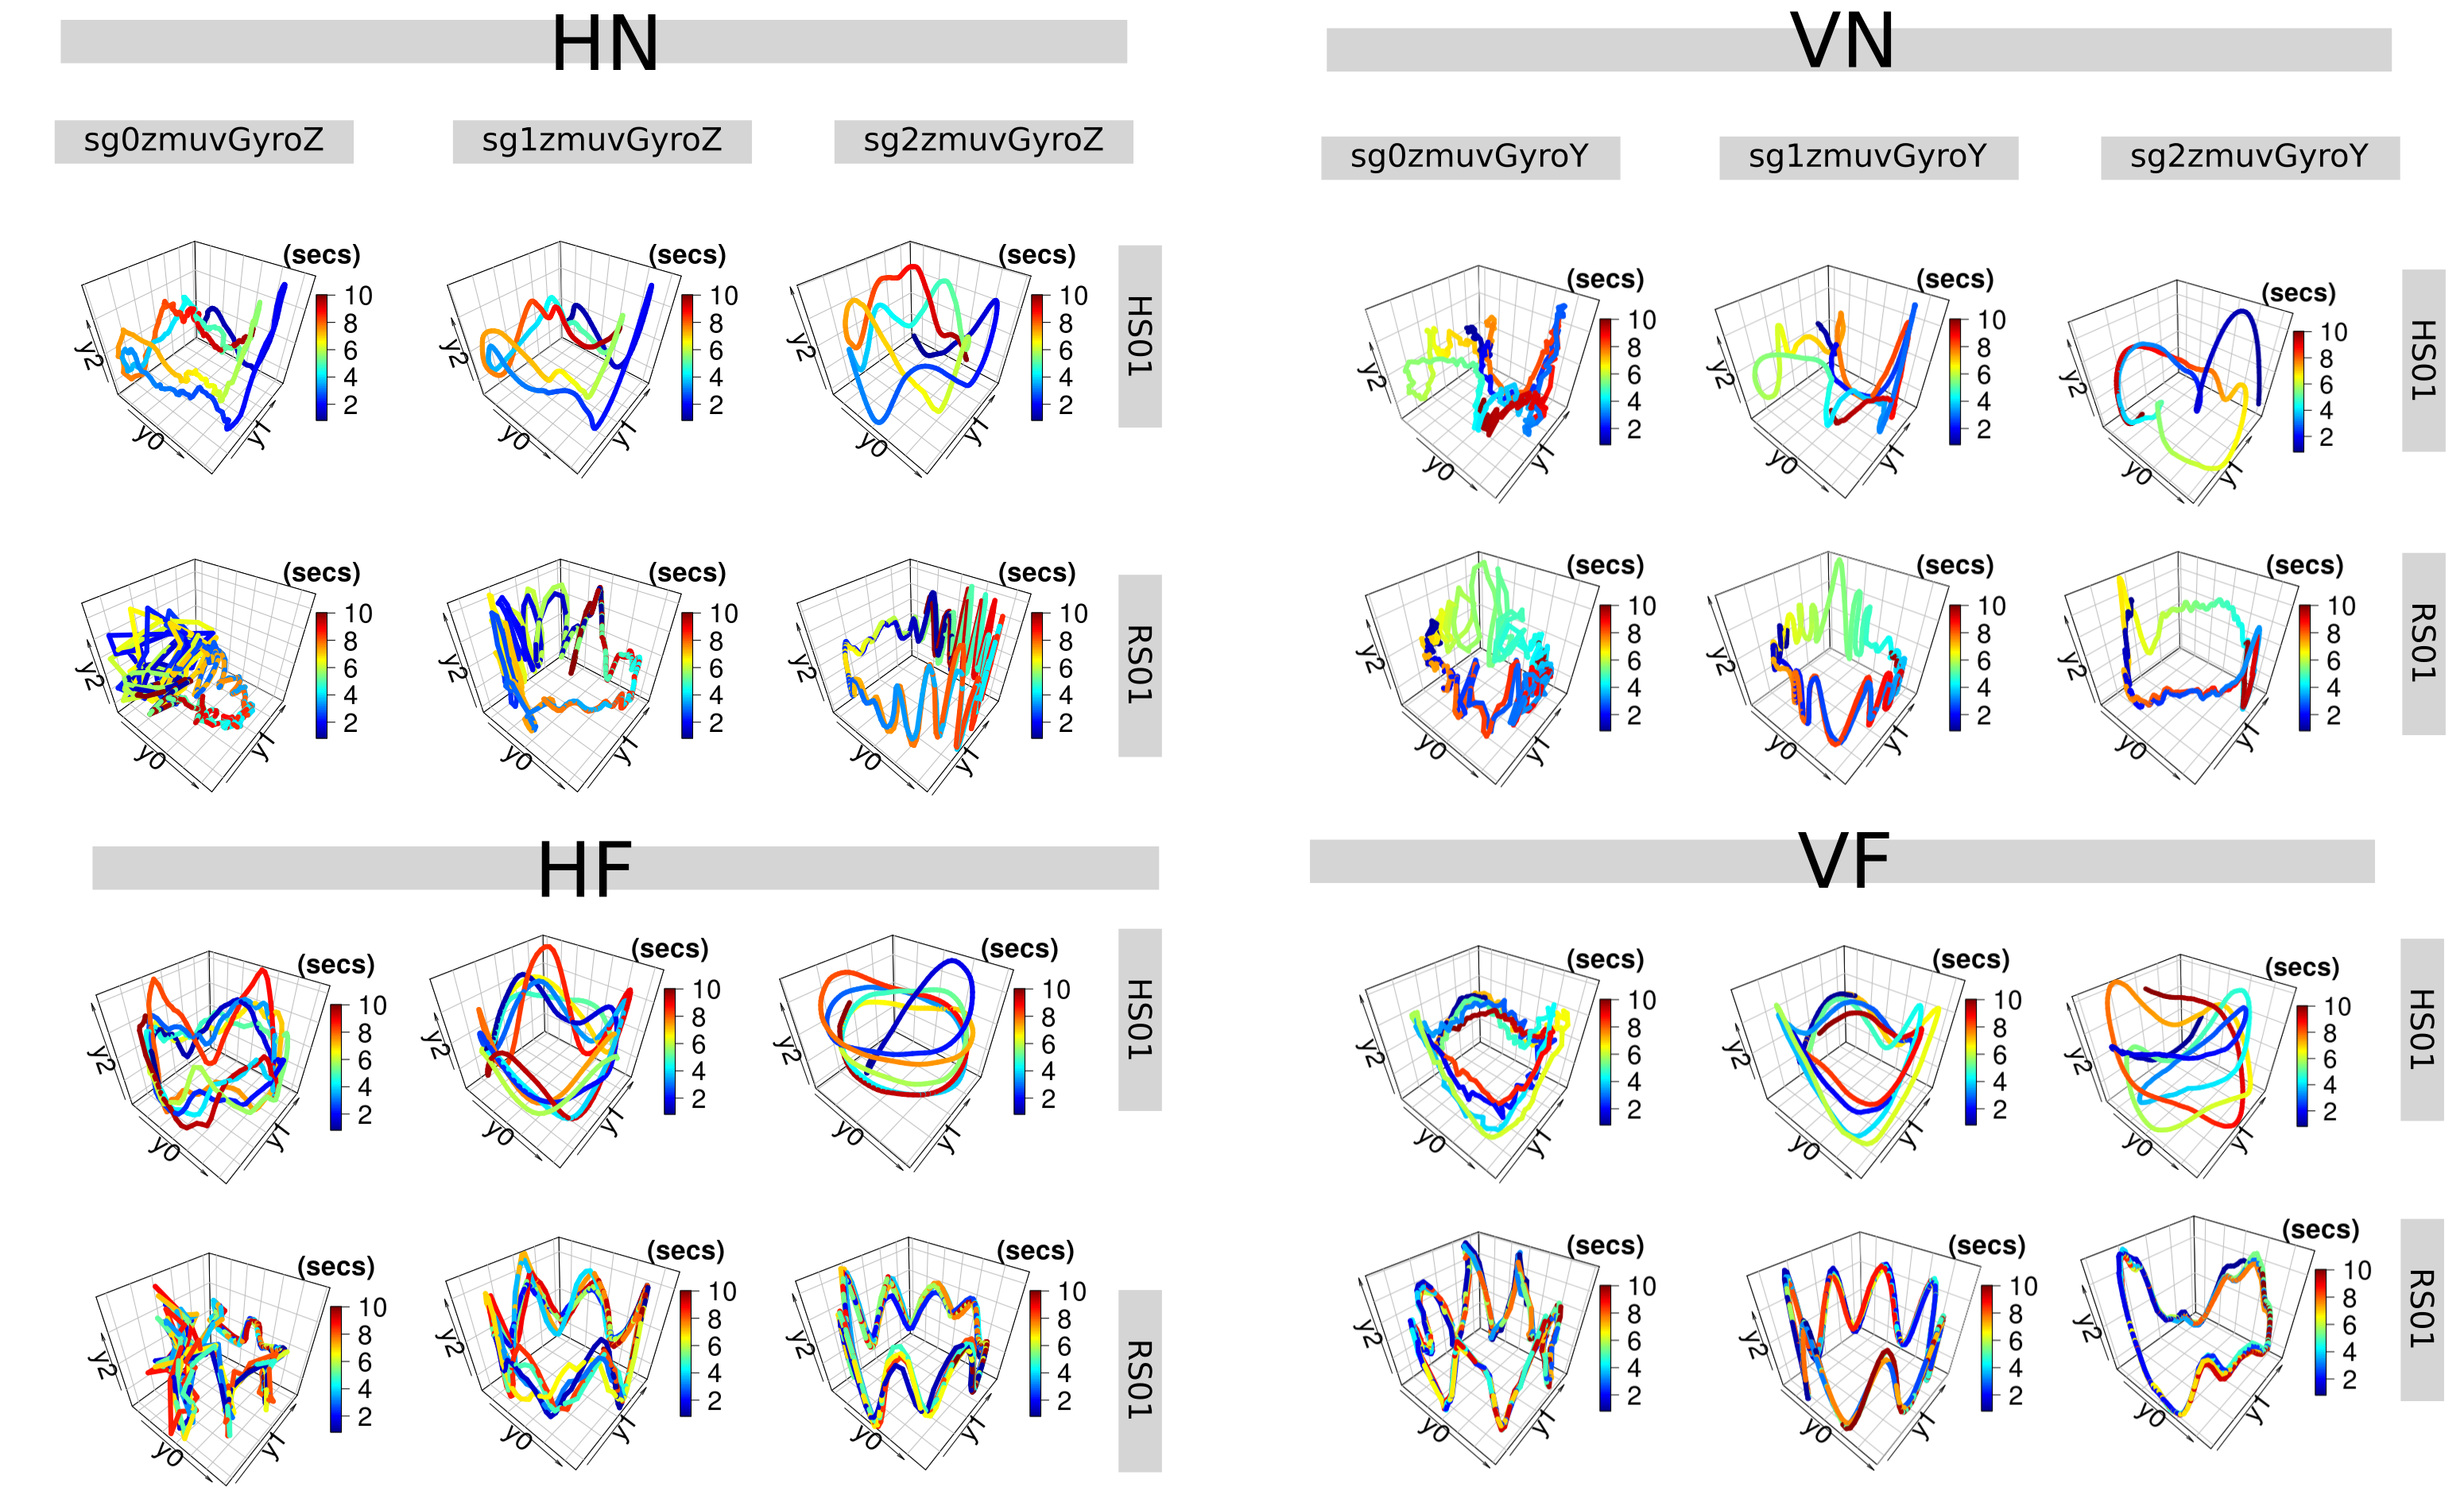
\includegraphics[width=0.8\linewidth]{./figs/results/ch6-rss/versions/drawing-v00}{}
	\caption{RSS for participant 01 computed with ($m=6$, $\tau=8$)
	for different activities, signals and source of time-series data.
	} 
   \end{figure}
\end{frame}
}





%%%%%%%%%%%%%%%%%%%%%%%%%%%%%%%%%%%%%%%%%%%%%%%%%%%%%%%
{
%\paper{Xochicale 2019 in {\bf PhD Thesis}}
\begin{frame}{Recurrence Plots}
    \begin{figure}
        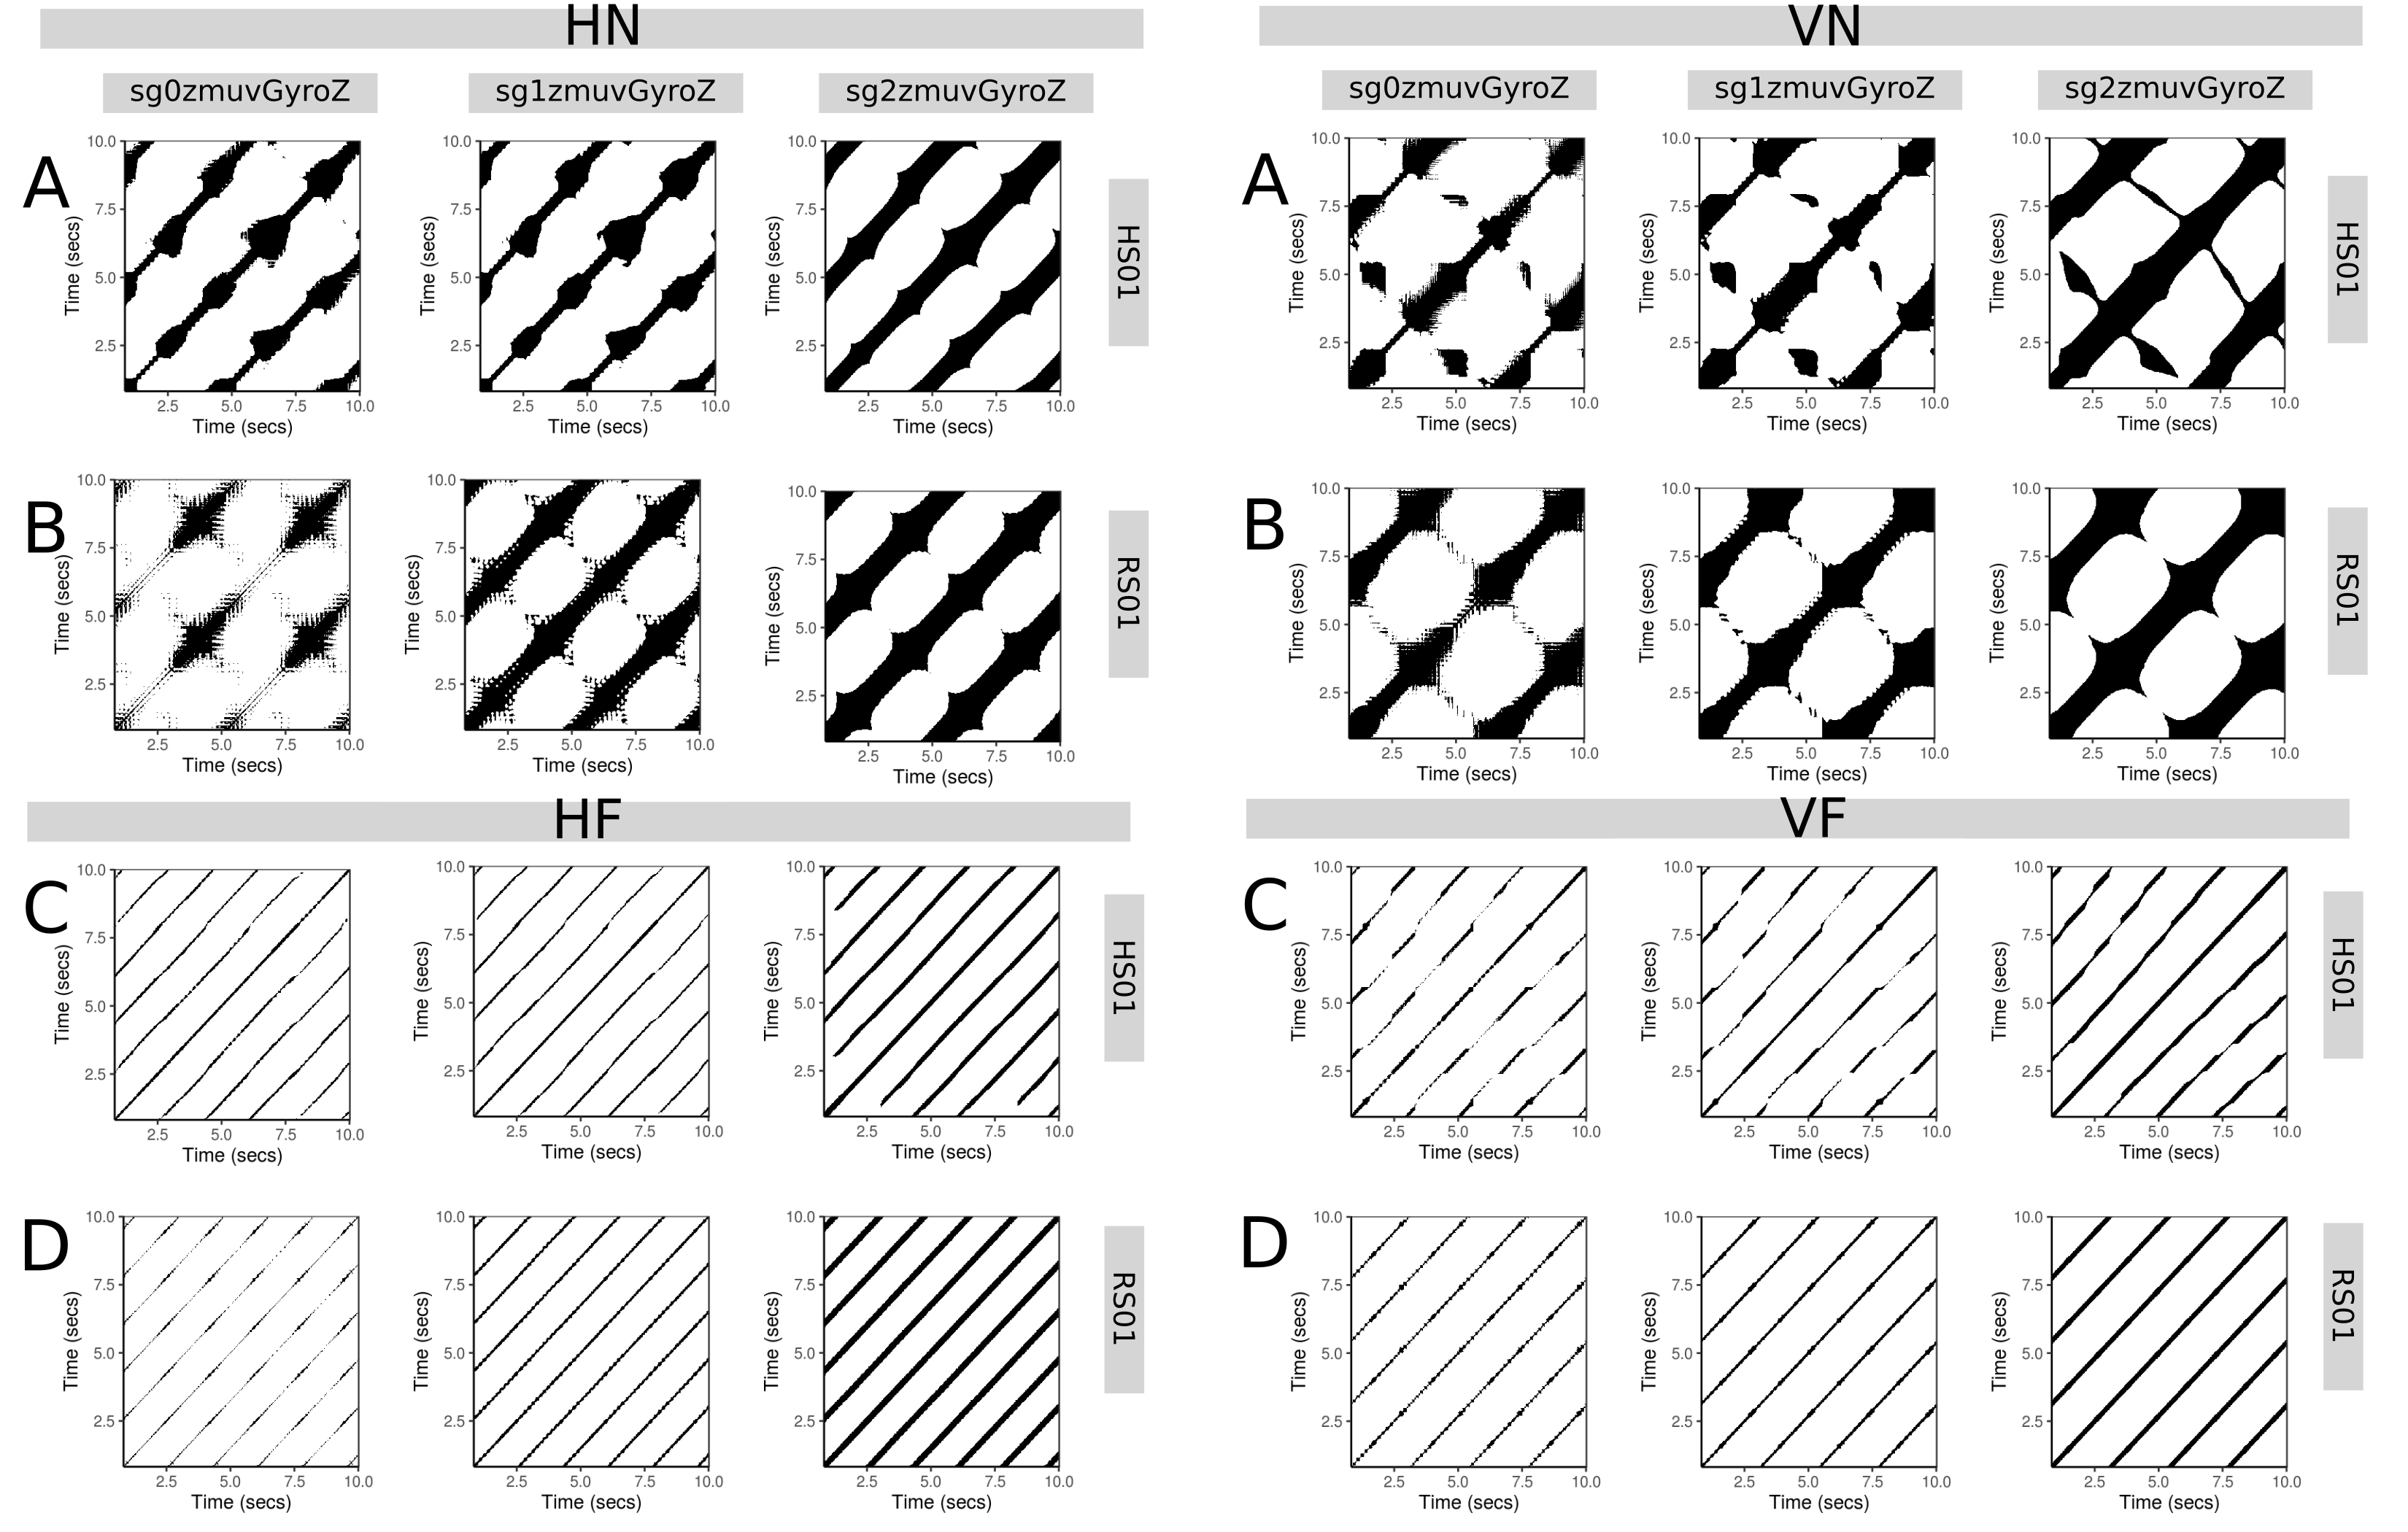
\includegraphics[width=0.8\linewidth]{./figs/results/ch6-rp/versions/drawing-v00}{}
	\caption{RP for participant 01 computed 
	with ($m=6$, $\tau=8$, $\epsilon=1$)
	for different activities, signals and source of time-series data.
	} 
   \end{figure}
	
\end{frame}
}




%%%%%%%%%%%%%%%%%%%%%%%%%%%%%%%%%%%%%%%%%%%%%%%%%%%%%%%
{
\paper{Xochicale 2019 in {\bf PhD Thesis}}

\begin{frame}{Recurrence Quantification Analysis}
    \begin{figure}
        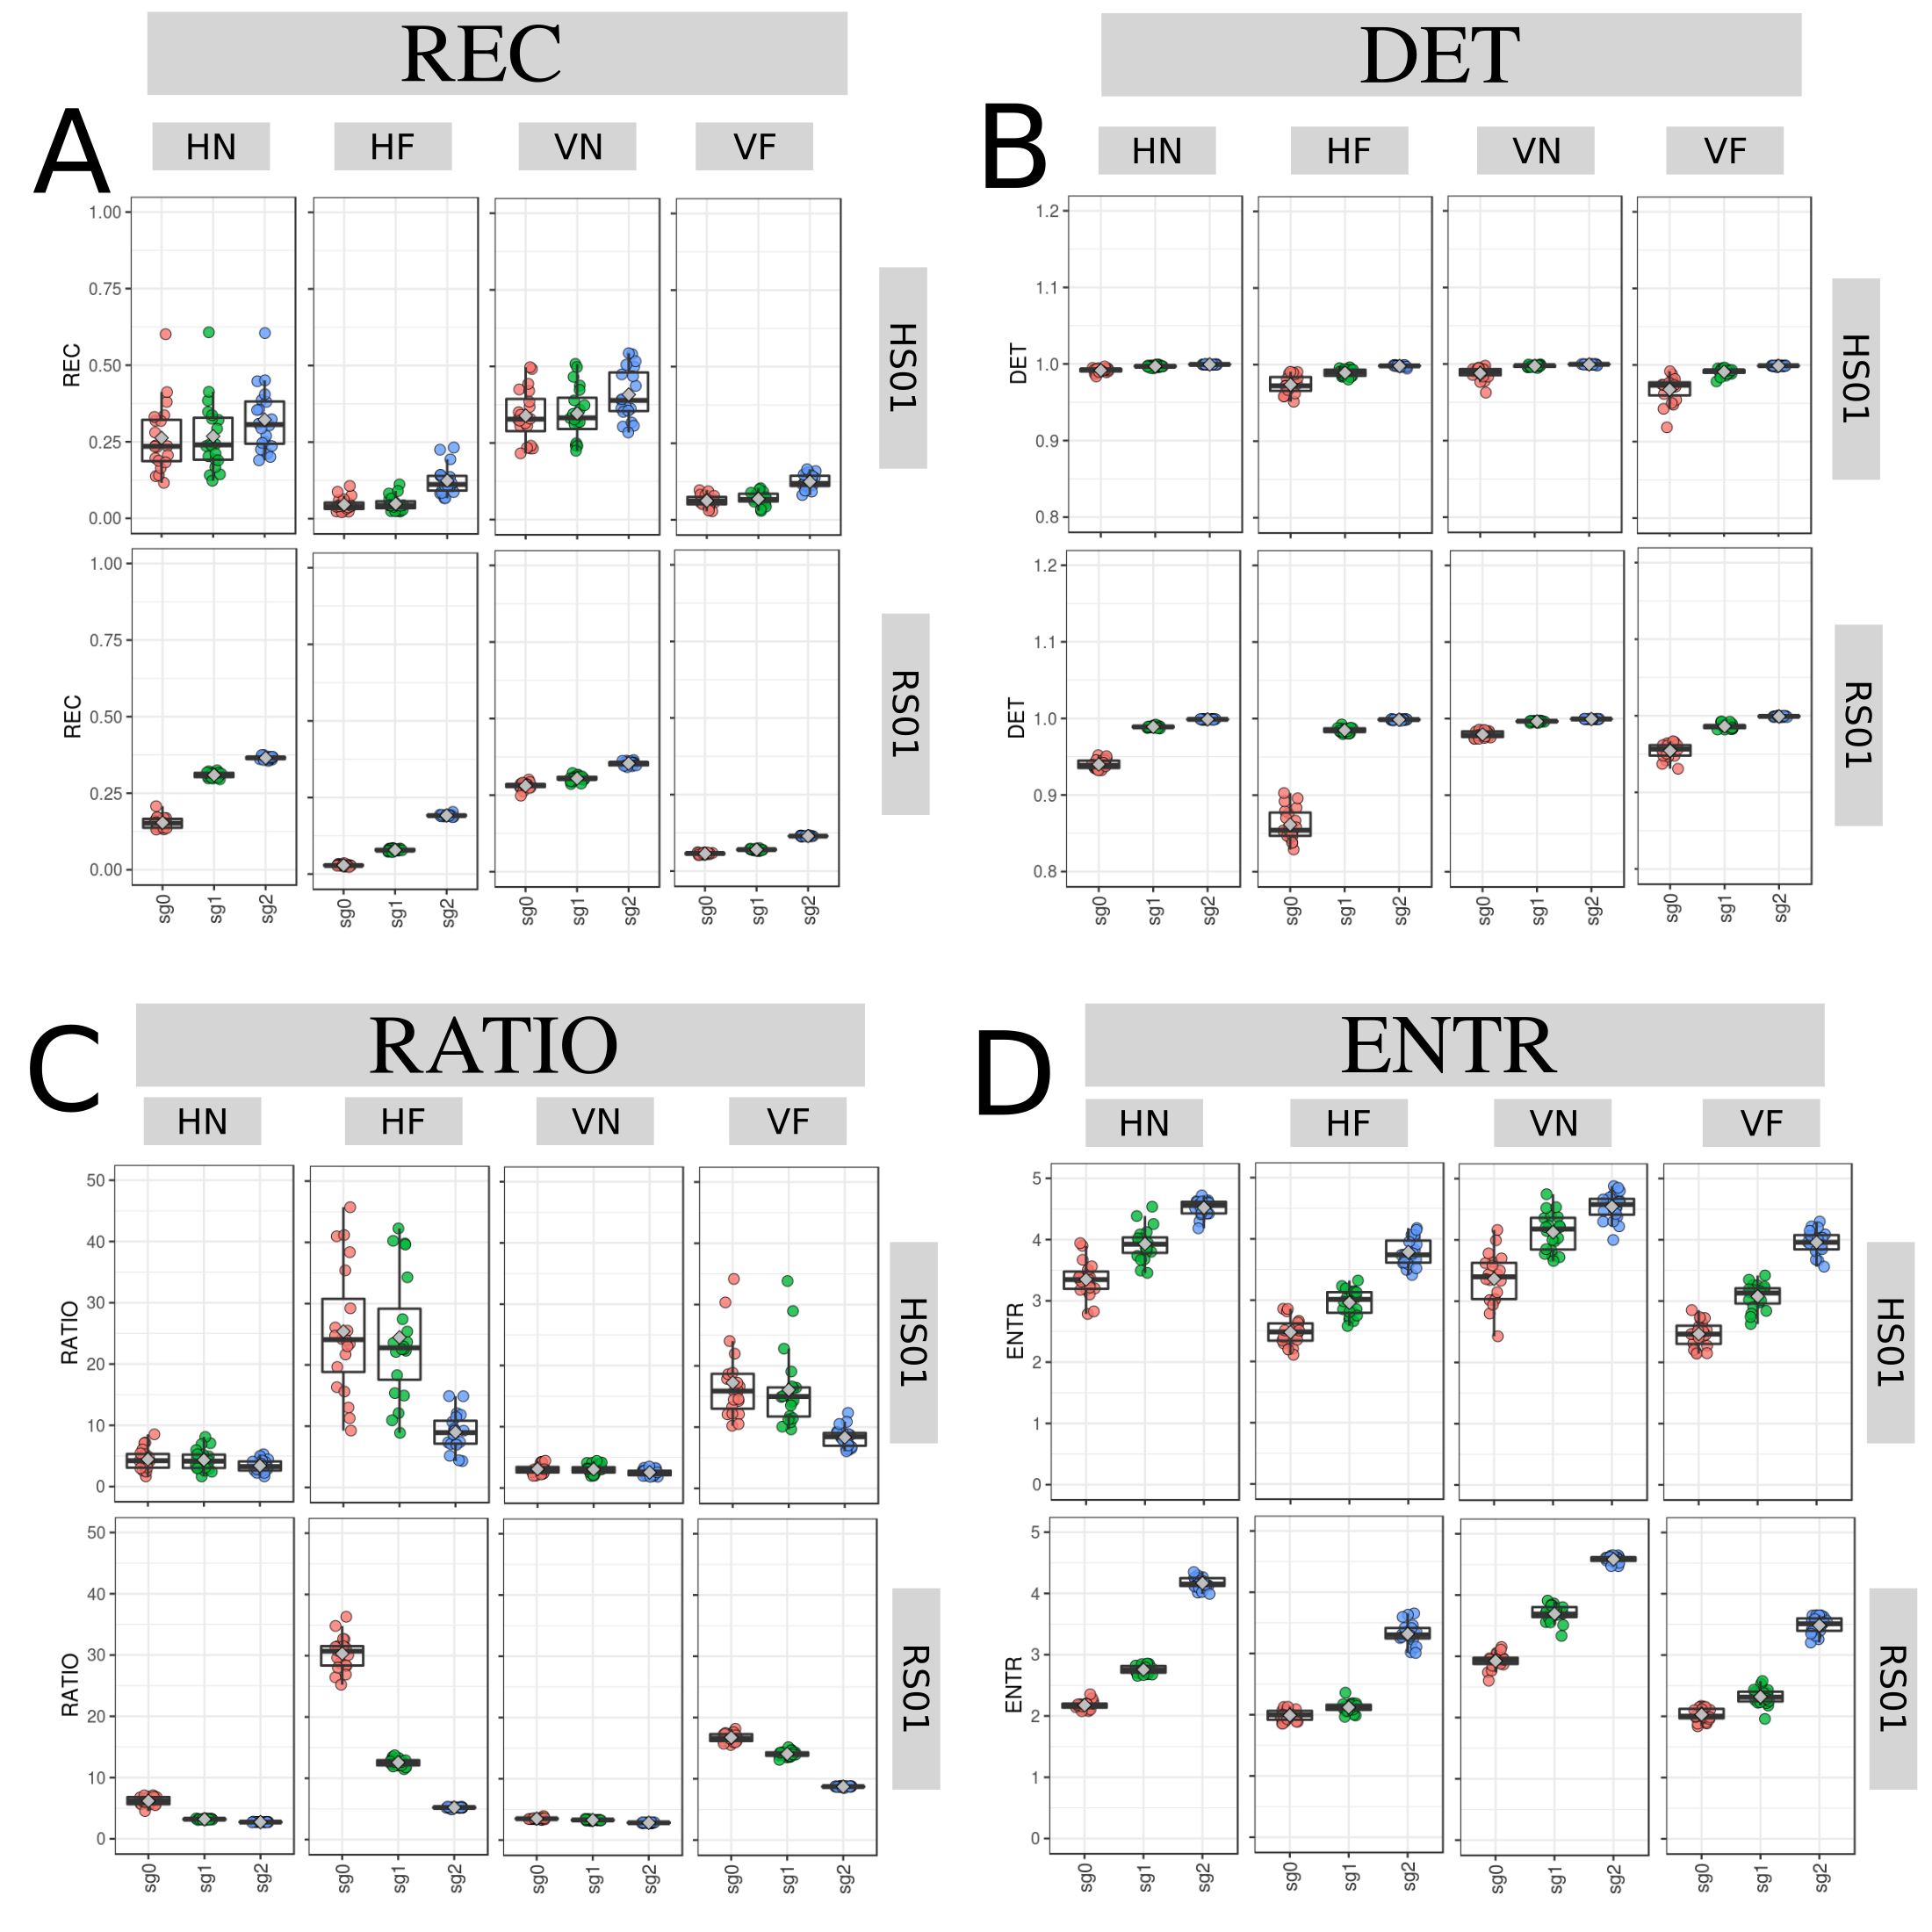
\includegraphics[width=0.45\linewidth]{./figs/results/ch6-rqa/versions/drawing-v00}{}
	\caption{Box values of  RQA computed with 
	($m=7$, $\tau=5$, $\epsilon=1$). 
	These values are for 20 participants.
} 
   \end{figure}
	
\end{frame}
}


%%%%%%%%%%%%%%%%%%%%%%%%%%%%%%%%%%%%%%%%%%%%%%%%%%%%%%%
{
\paper{Xochicale 2019 in {\bf PhD Thesis}}

\begin{frame}{RQA ENTR for $\epsilon$ thresholds
	\& smoothness
}
    \begin{figure}
        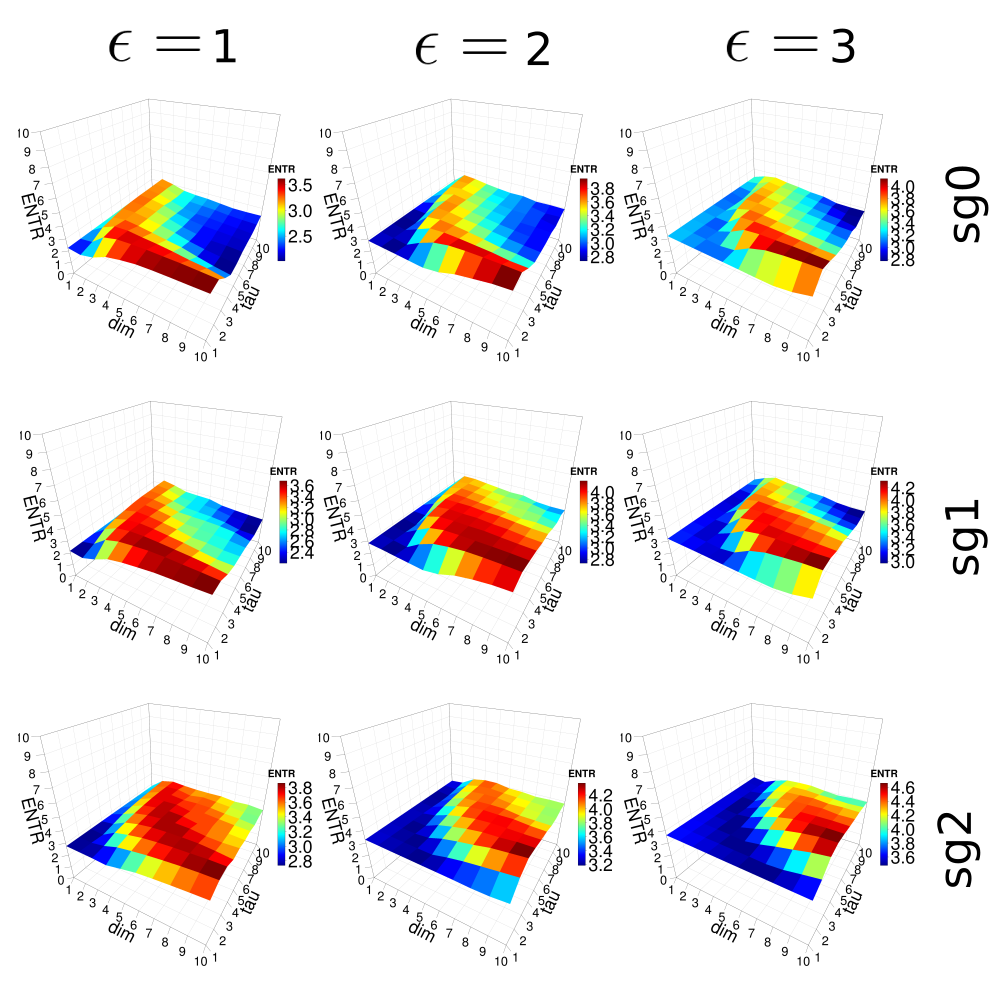
\includegraphics[width=0.45\linewidth]{./figs/results/rqa-epsilons/versions/drawing-v00}{}
	\caption{
	RQA ENTR values are for
	$p03$, sensor $HS01$, of a window size of 10-secs (500 samples).
} 
   \end{figure}
	
\end{frame}
}



%%%%%%%%%%%%%%%%%%%%%%%%%%%%%%%%%%%%%%%%%%%%%%%%%%%%%%%
{
\paper{Xochicale 2019 in {\bf PhD Thesis}}

\begin{frame}{RQA ENTR for sensors and activities
}
    \begin{figure}
        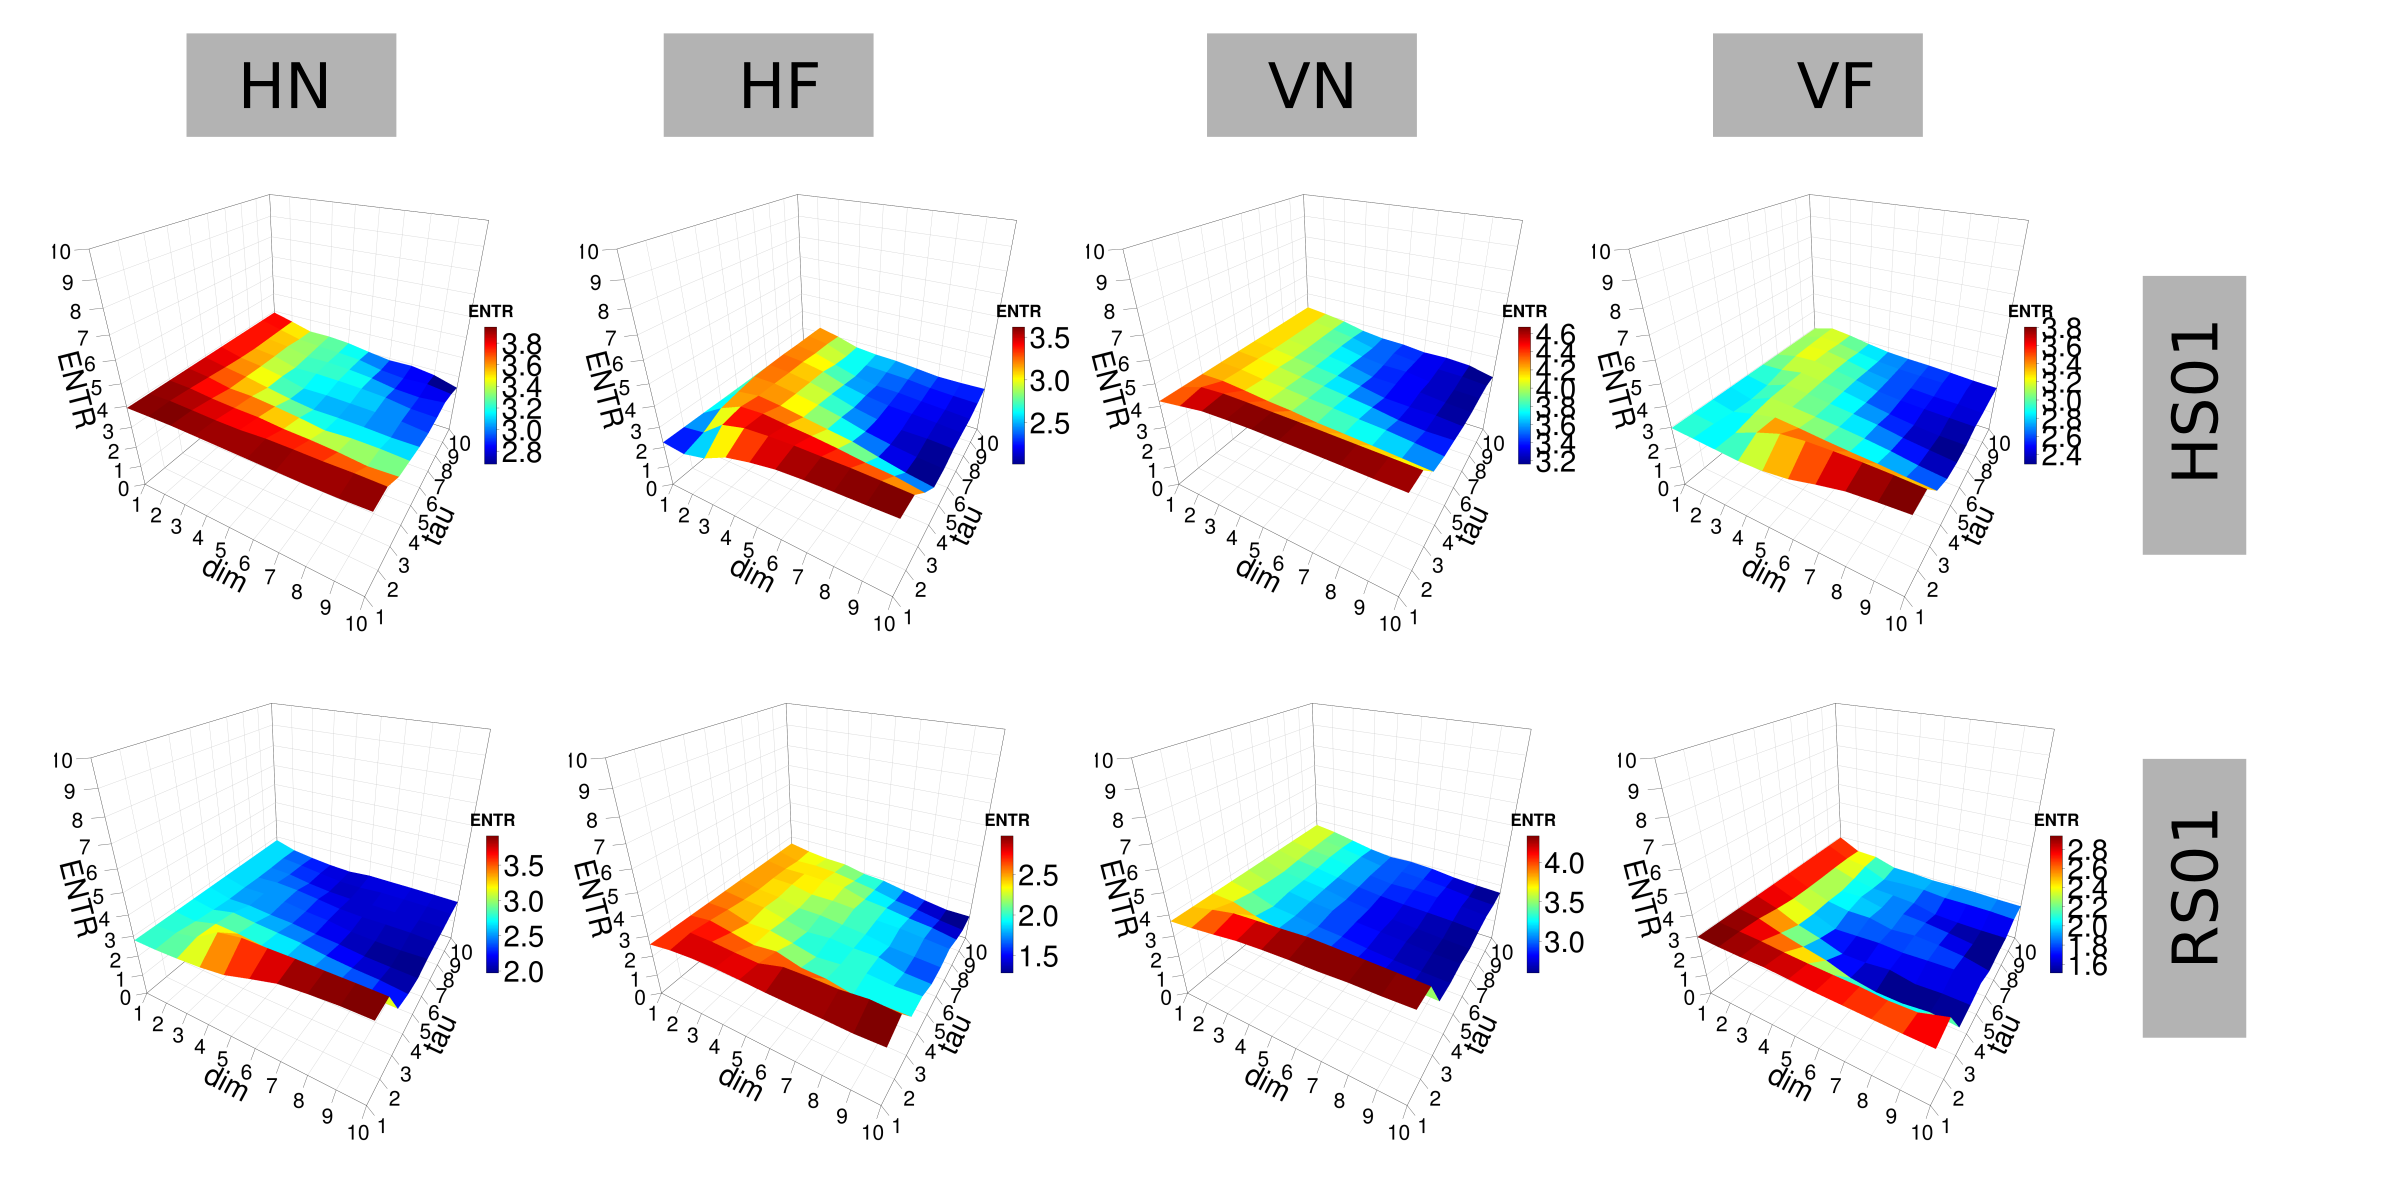
\includegraphics[width=0.75\linewidth]{./figs/results/rqa-epsilons-sensors-activities/versions/drawing-v00}{}
	\caption{
	RQA ENTR values are for
	$p03$, $sg0$ and window size of 10-secs (500 samples).
} 
   \end{figure}
	
\end{frame}
}







\subsection{}
%%%%%%%%%%%%%%%%%%%%%%%%%%%%%%%%%%%%%%%%%%%%%%%%%%%%%%%
{
\paper{Xochicale 2019 in {\bf PhD Thesis}}

\begin{frame}{Window size lengths
}
   \begin{figure}
        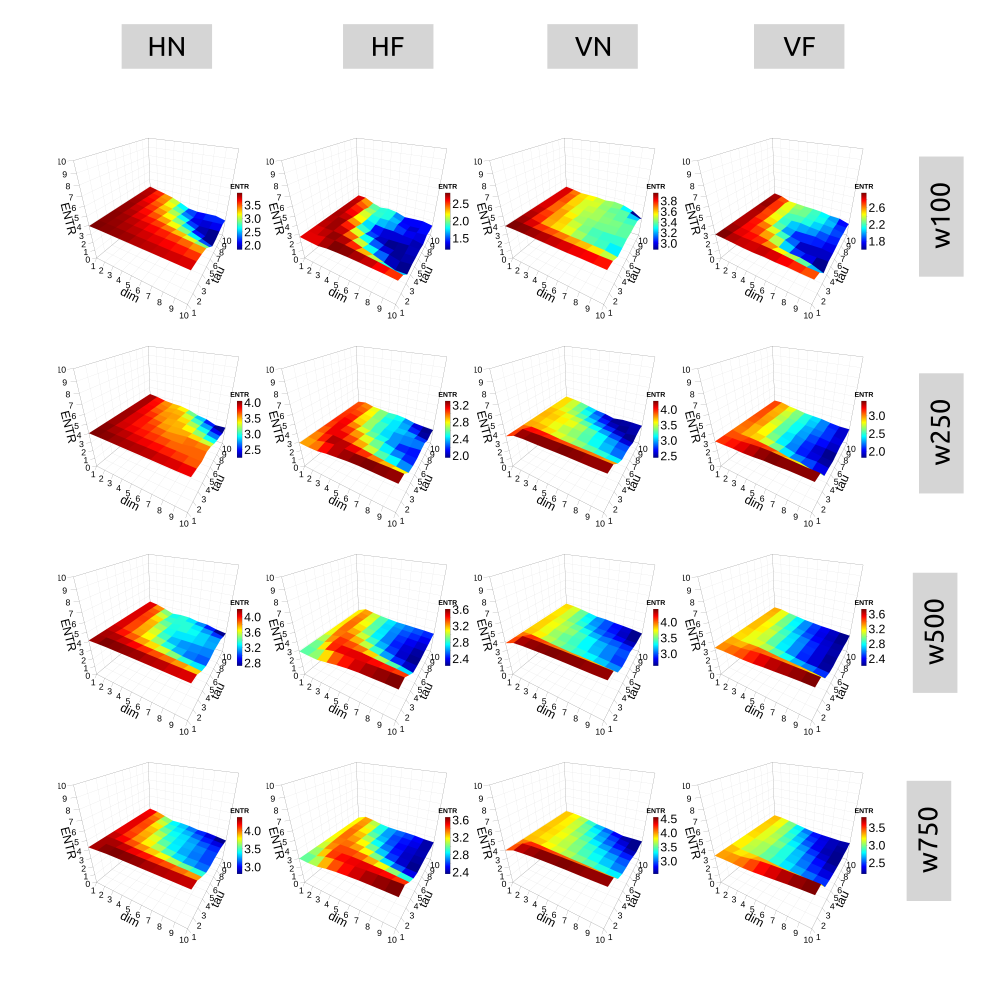
\includegraphics[width=0.55\linewidth]{./figs/results/3d-rqa-epsilons-windows/versions/drawing-v00}{}
	\caption{Window length size effect on 3D surface plots of RQA.} 
   \end{figure}
	
\end{frame}
}









\subsection{}
%%%%%%%%%%%%%%%%%%%%%%%%%%%%%%%%%%%%%%%%%%%%%%%%%%%%%%%
{
\paper{Xochicale 2019 in {\bf PhD Thesis}}

\begin{frame}{Participants
}
    \begin{figure}
        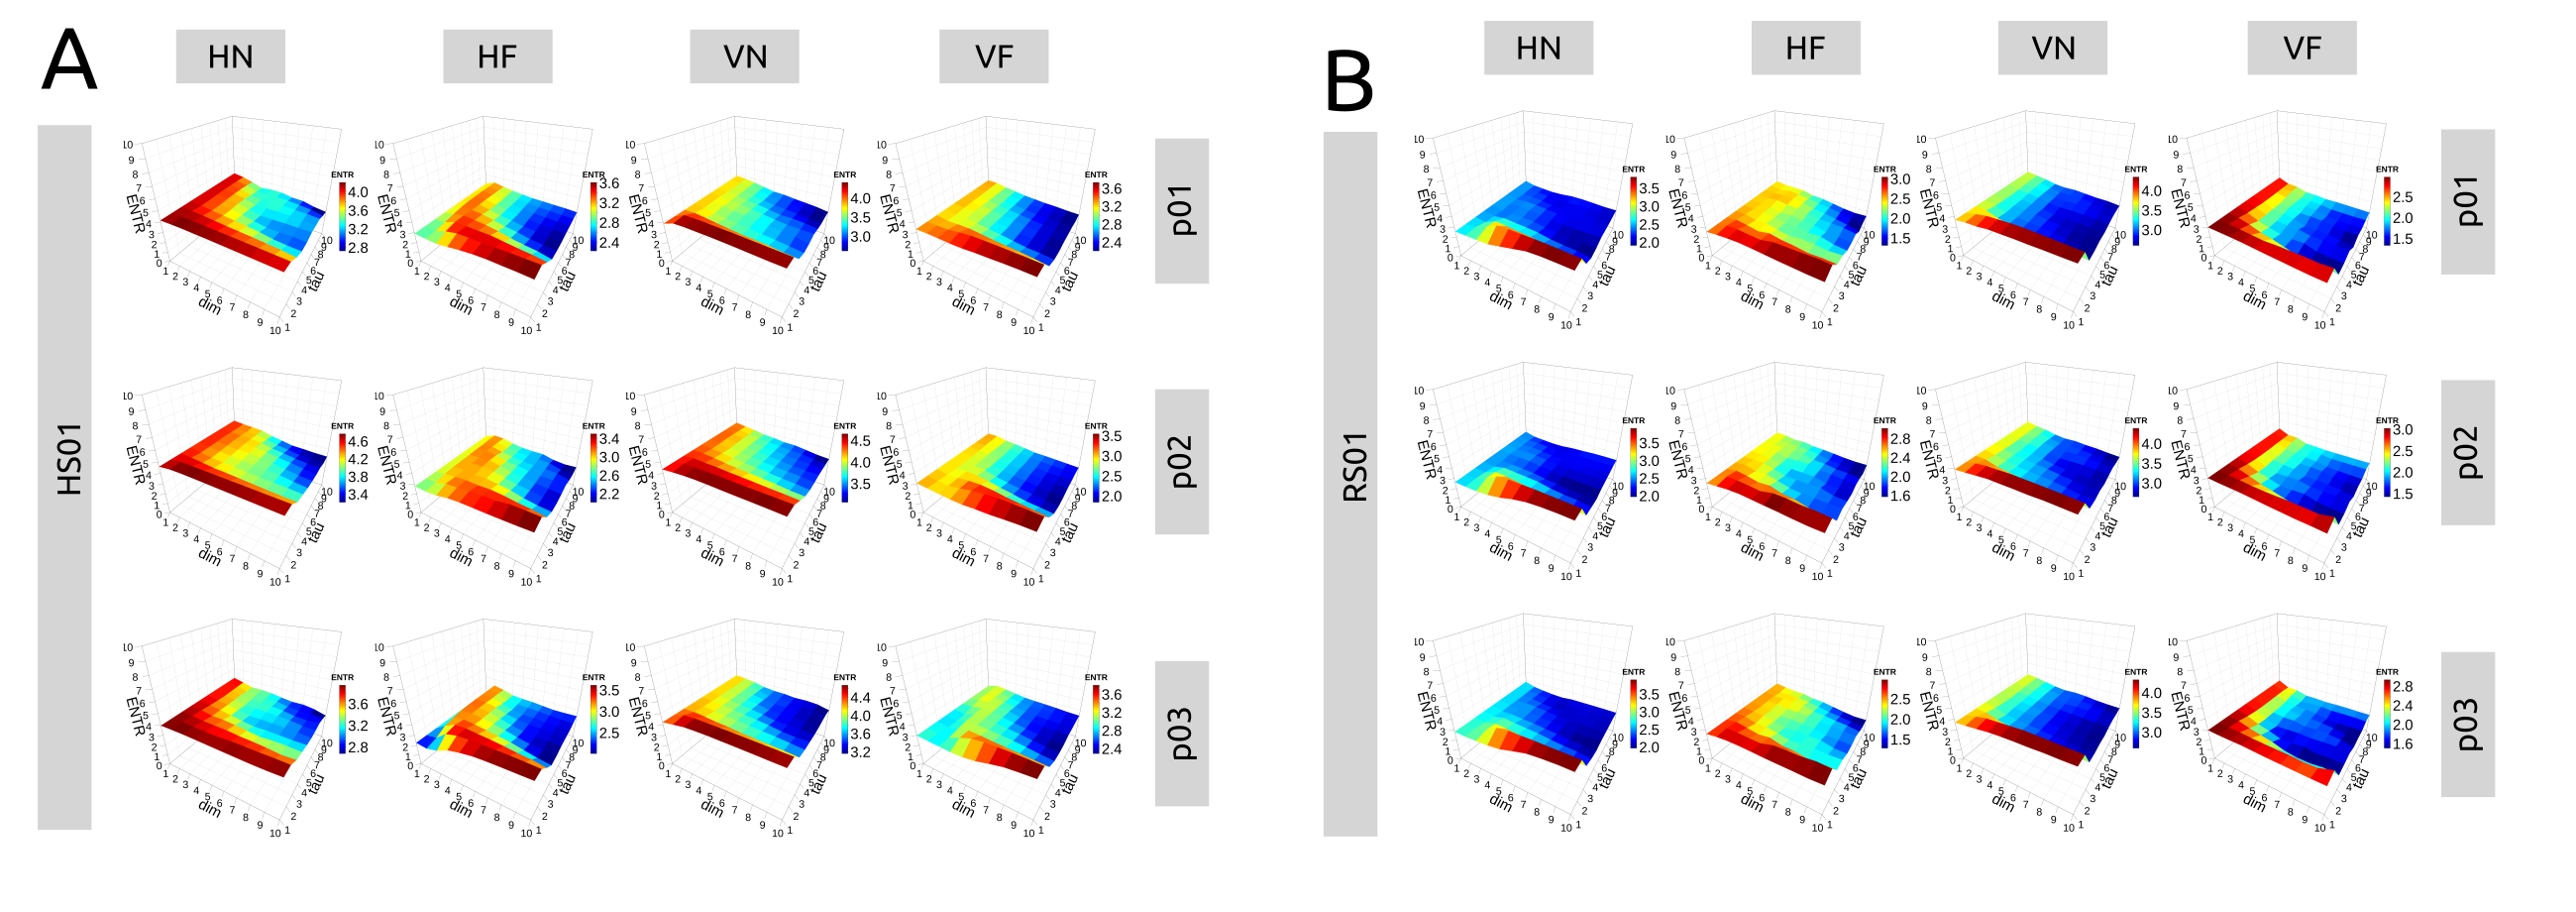
\includegraphics[width=1.0\linewidth]{./figs/results/3d-rqa-epsilons-participants/versions/drawing-v00}{}
	\caption{Participants differences of 3D surface plots of RQA.} 
   \end{figure}
	
\end{frame}
}


%%%%%%%%%%%%%%%%%%%%%%%%%%%%%%%%%%%%%%%%%%%%%%%%%%%%%%%%%
%{
%\paper{Xochicale 2019 in {\bf PhD Thesis}}
%
%\begin{frame}{3D surfaces plots of RQA
%	{\bf (in preparation)}
%}
%    \begin{figure}
%        \centering
%        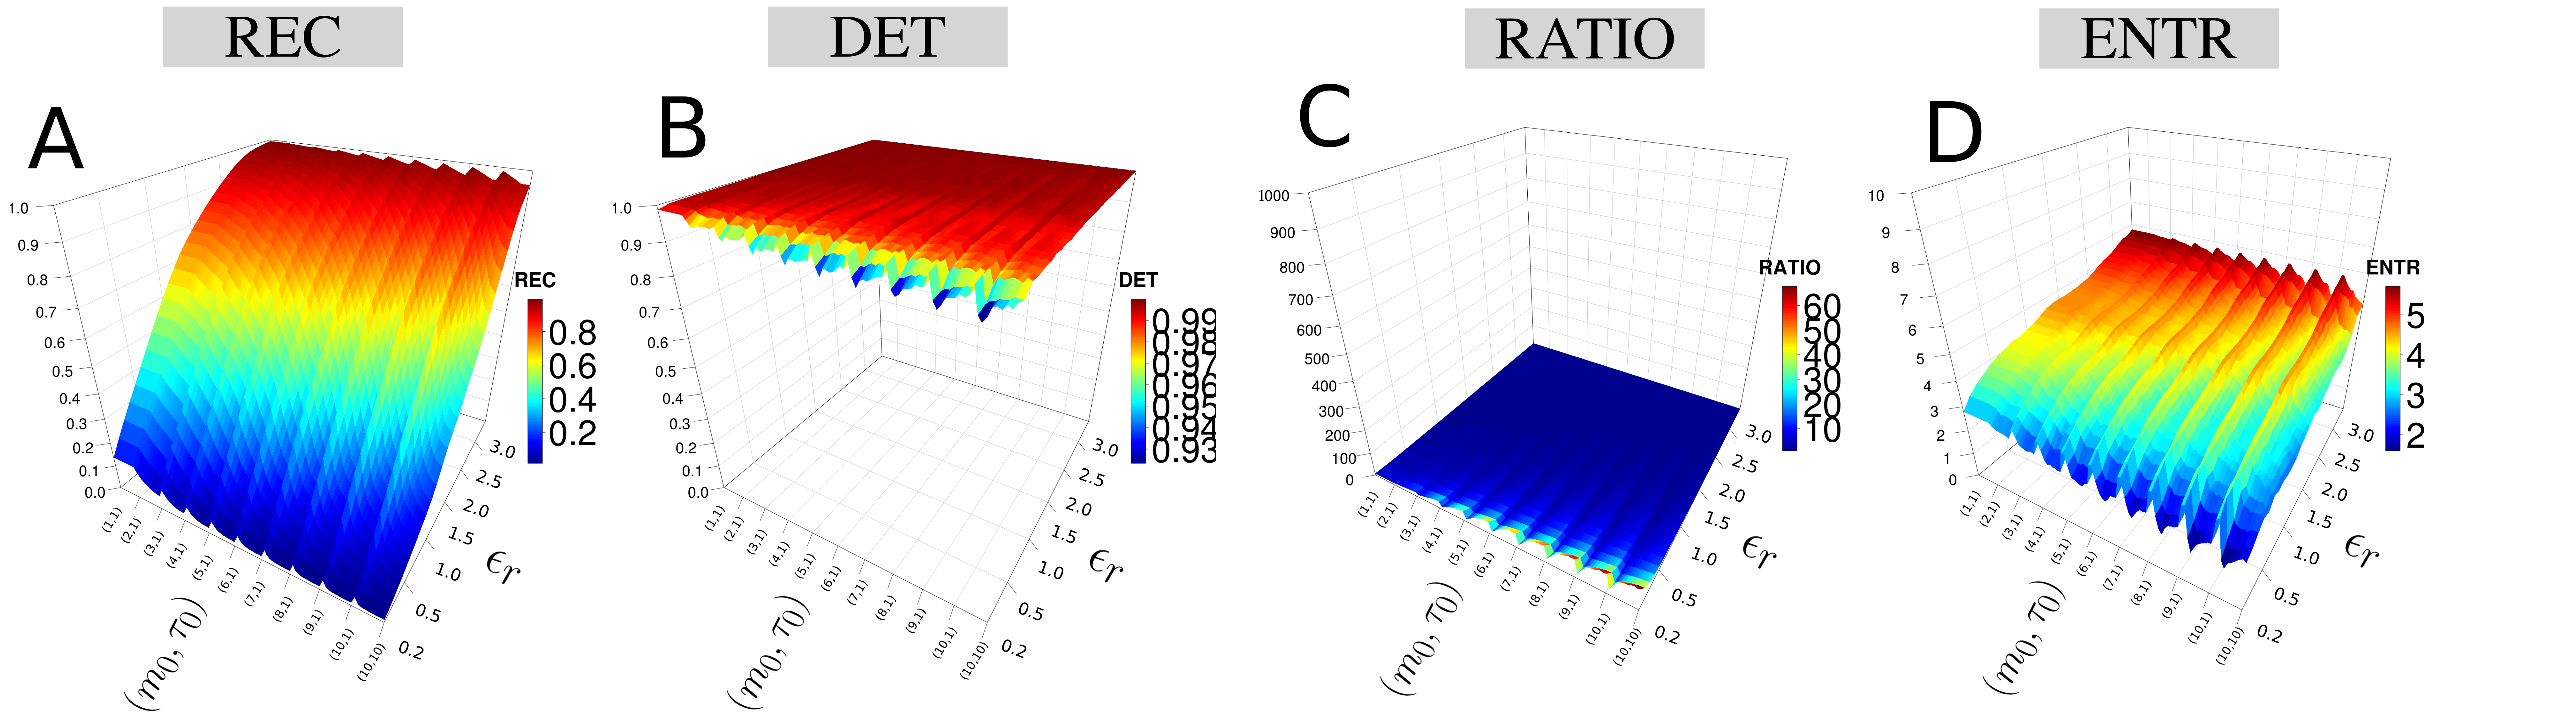
\includegraphics[width=0.75\linewidth]{./figs/results/3d-rqa/versions/drawing-v00}{}
%	\small
%	\caption{
%		3D RQA surfaces 
%	with increasing pair of embedding parameters 
%	($0 \le m \le 10$, $0 \le \tau \le 10$) 
%	and recurrence thresholds ($ 0.2 \le \epsilon \le 3 $).
%	} 
%   \end{figure}
%	
%\end{frame}
%}
%
